\begin{frame}
\frametitle{Change in perspective}
%\begin{columns}[c] % The "c" option specifies centered vertical alignment while the "t" option is used for top vertical alignment

%\column{.3\textwidth} % Left column and width
%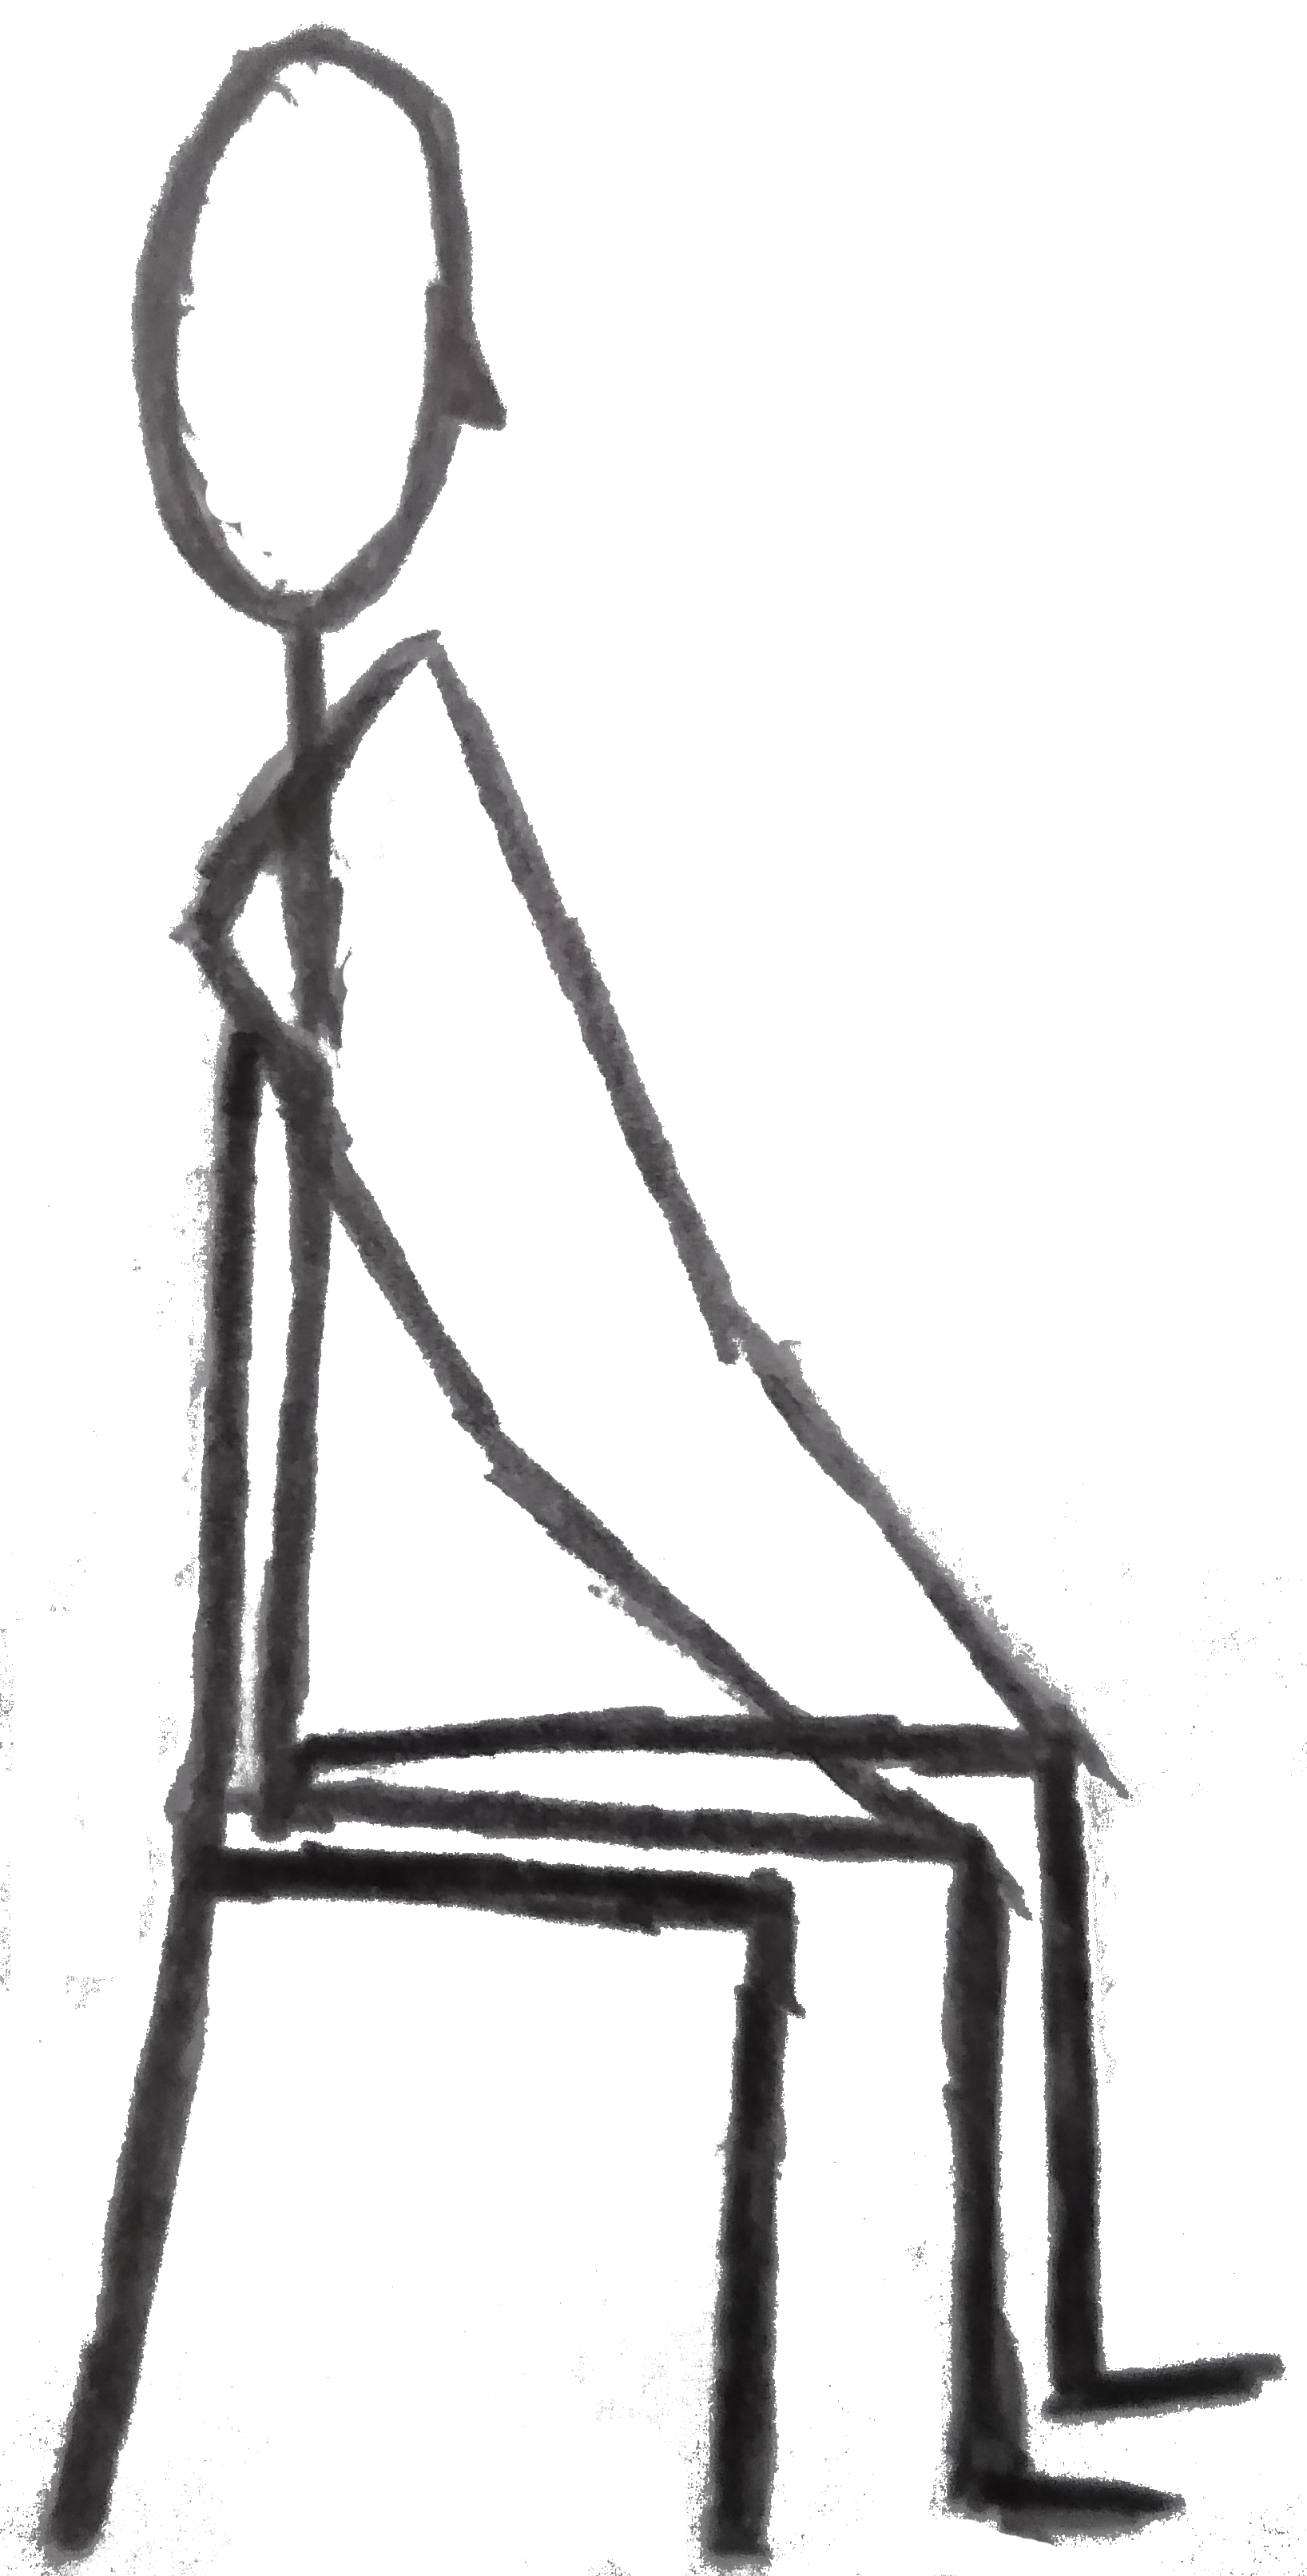
\includegraphics[width=\linewidth]{Sitting_chair_side.png}
%\column{.7\textwidth} % Right column and width
\begin{itemize}
\item You become more more \structure{steady and confident}.
\item Your motivation to \structure{take care of yourself} will increase.
\item Your confidence in your capacity to \structure{act in difficult situations appropriately} will improve.
\item You will feel a stronger readiness to \structure{see difficult situations as challenge} instead of a threat.
\item The most important: \structure{life will gain in content and sense}.
\end{itemize} 

%\end{columns}
\end{frame}
%------------------------------------------------------------
\begin{frame}
\frametitle{Relationship to pain and negative emotions}
%\begin{columns}[c] % The "c" option specifies centered vertical alignment while the "t" option is used for top vertical alignment

%\column{.3\textwidth} % Left column and width
%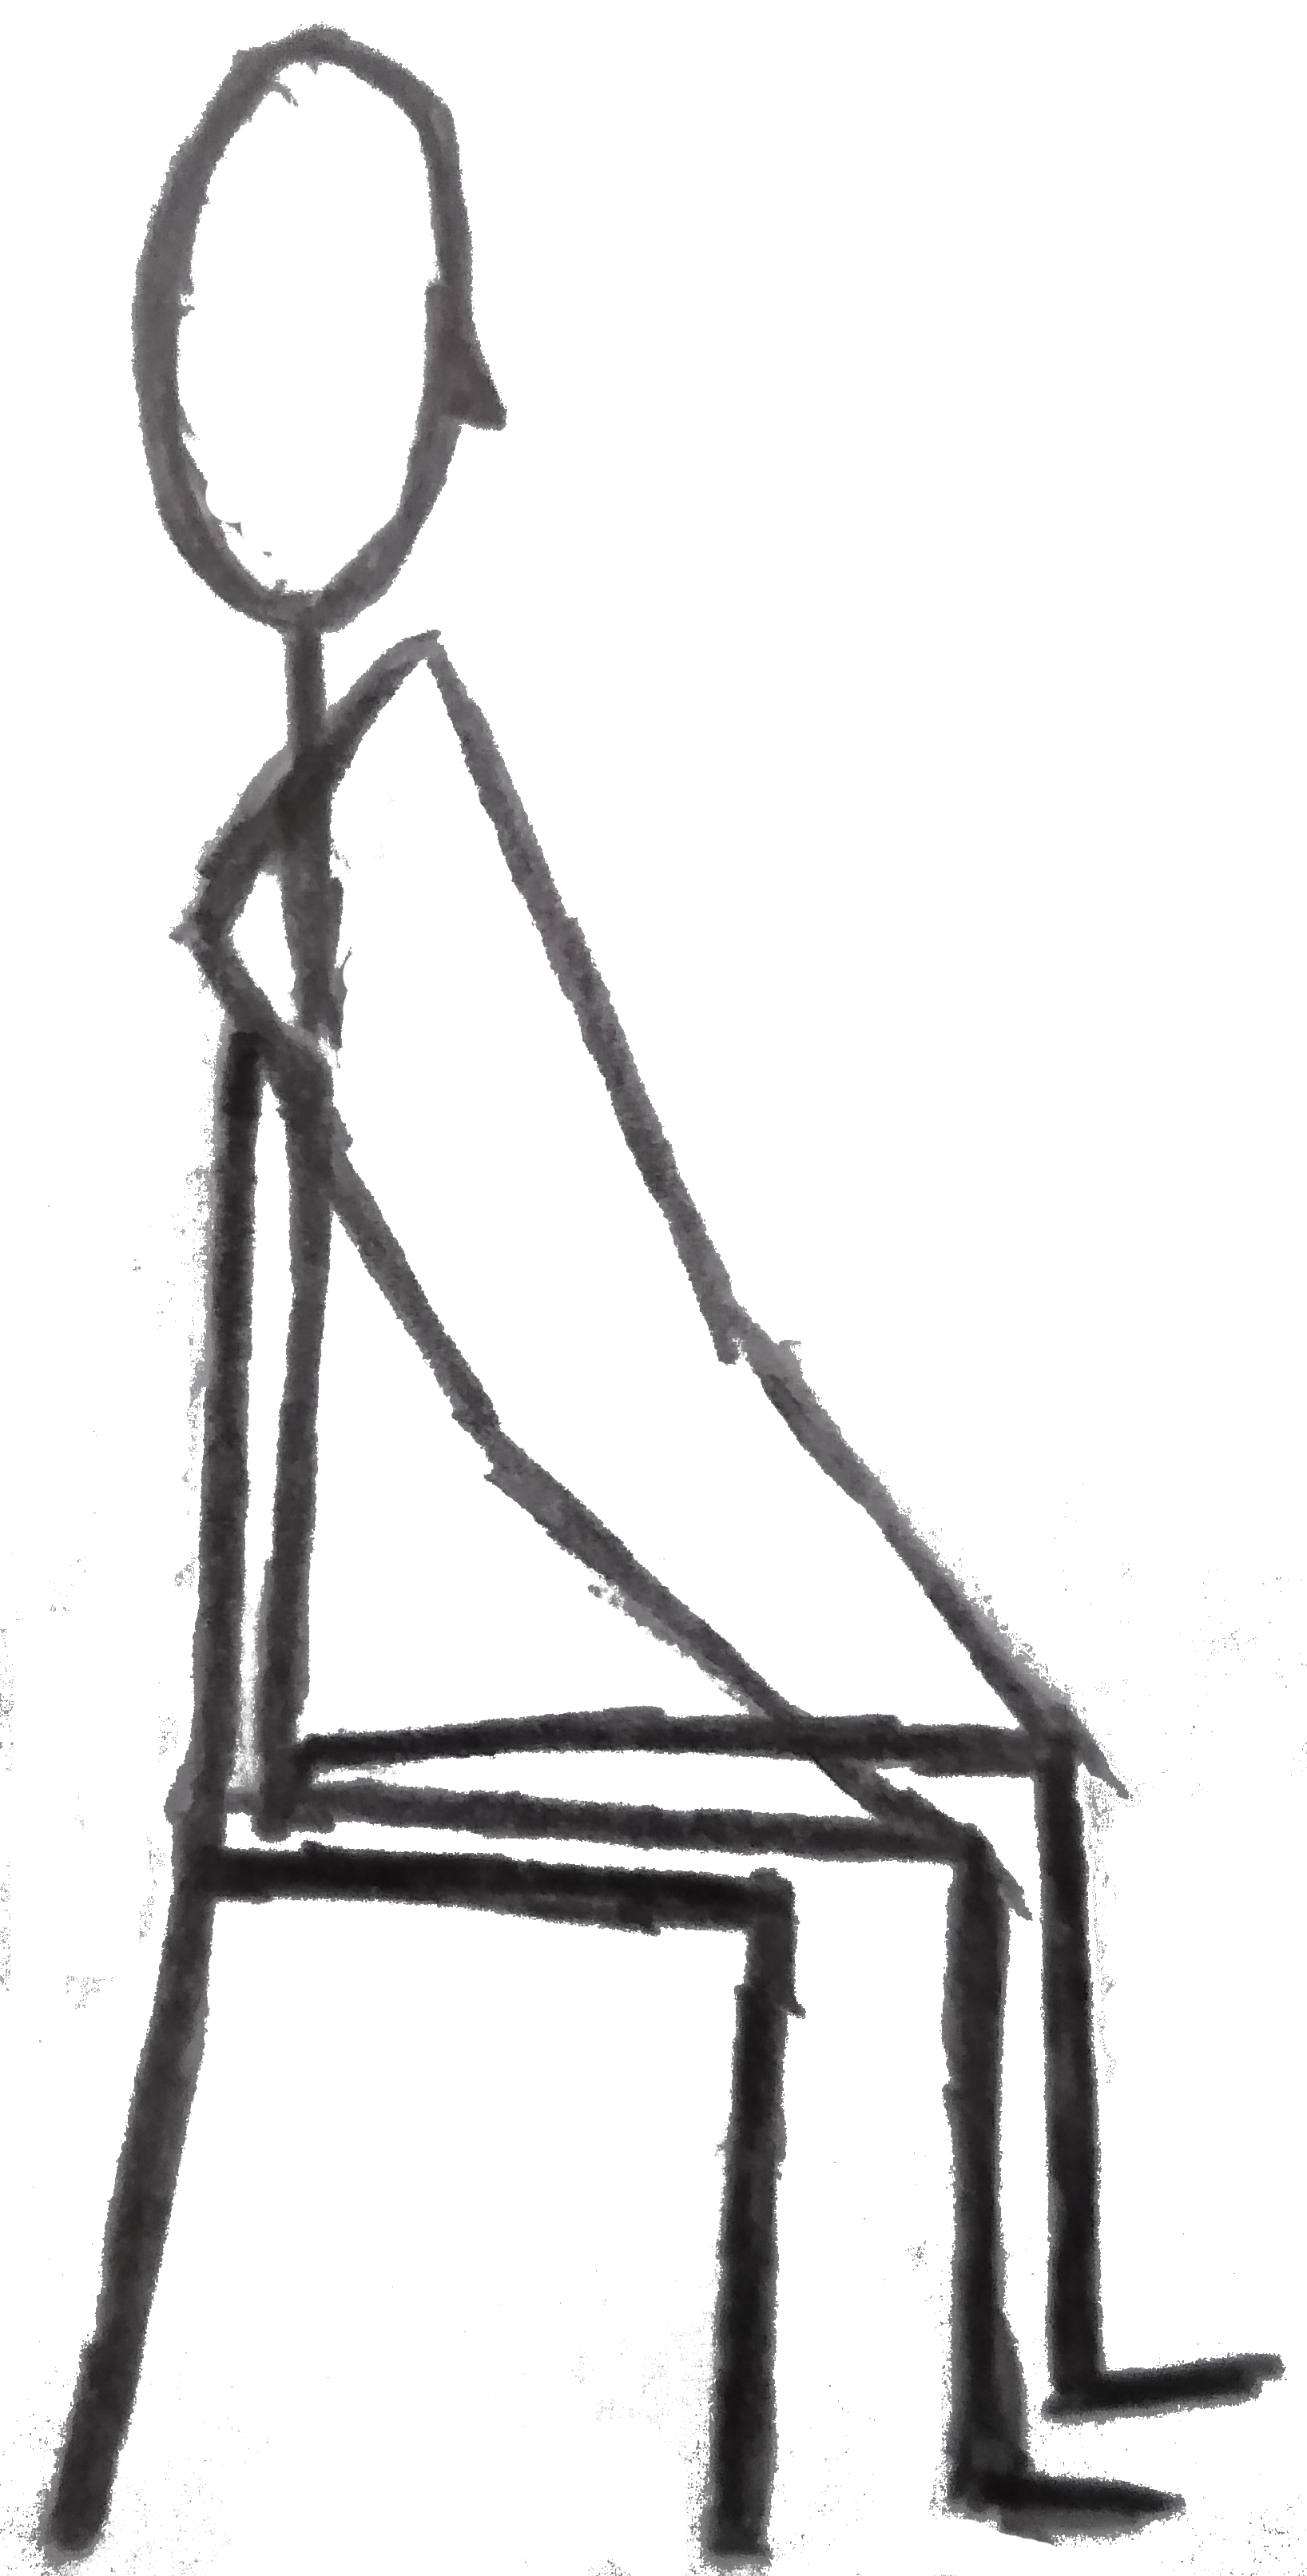
\includegraphics[width=\linewidth]{Sitting_chair_side.png}
%\column{.7\textwidth} % Right column and width


The practice of the body scan allows you to hold your \structure{focus for a prolonged time} and target it precisely. That improves your \structure{capacity to focus} and to concentrate and helps you to develop mindfulness and a precursor to the \structure{inner calm}. The body scan becomes most effective by being practiced \structure{daily over several weeks}.

Something about the \structure{relationship to pain or negative emotions changes} by approaching them with the intention to \structure{only perceive}, \structure{breathe} with them and let yourself \structure{sink into them}; by the simple act of \structure{turn towards them}, without evading right away.

%\end{columns}
\end{frame}
%------------------------------------------------------------
%------------------------------------------------------------
\begin{frame}
\frametitle{How}
%\begin{columns}[c] % The "c" option specifies centered vertical alignment while the "t" option is used for top vertical alignment

%\column{.3\textwidth} % Left column and width
%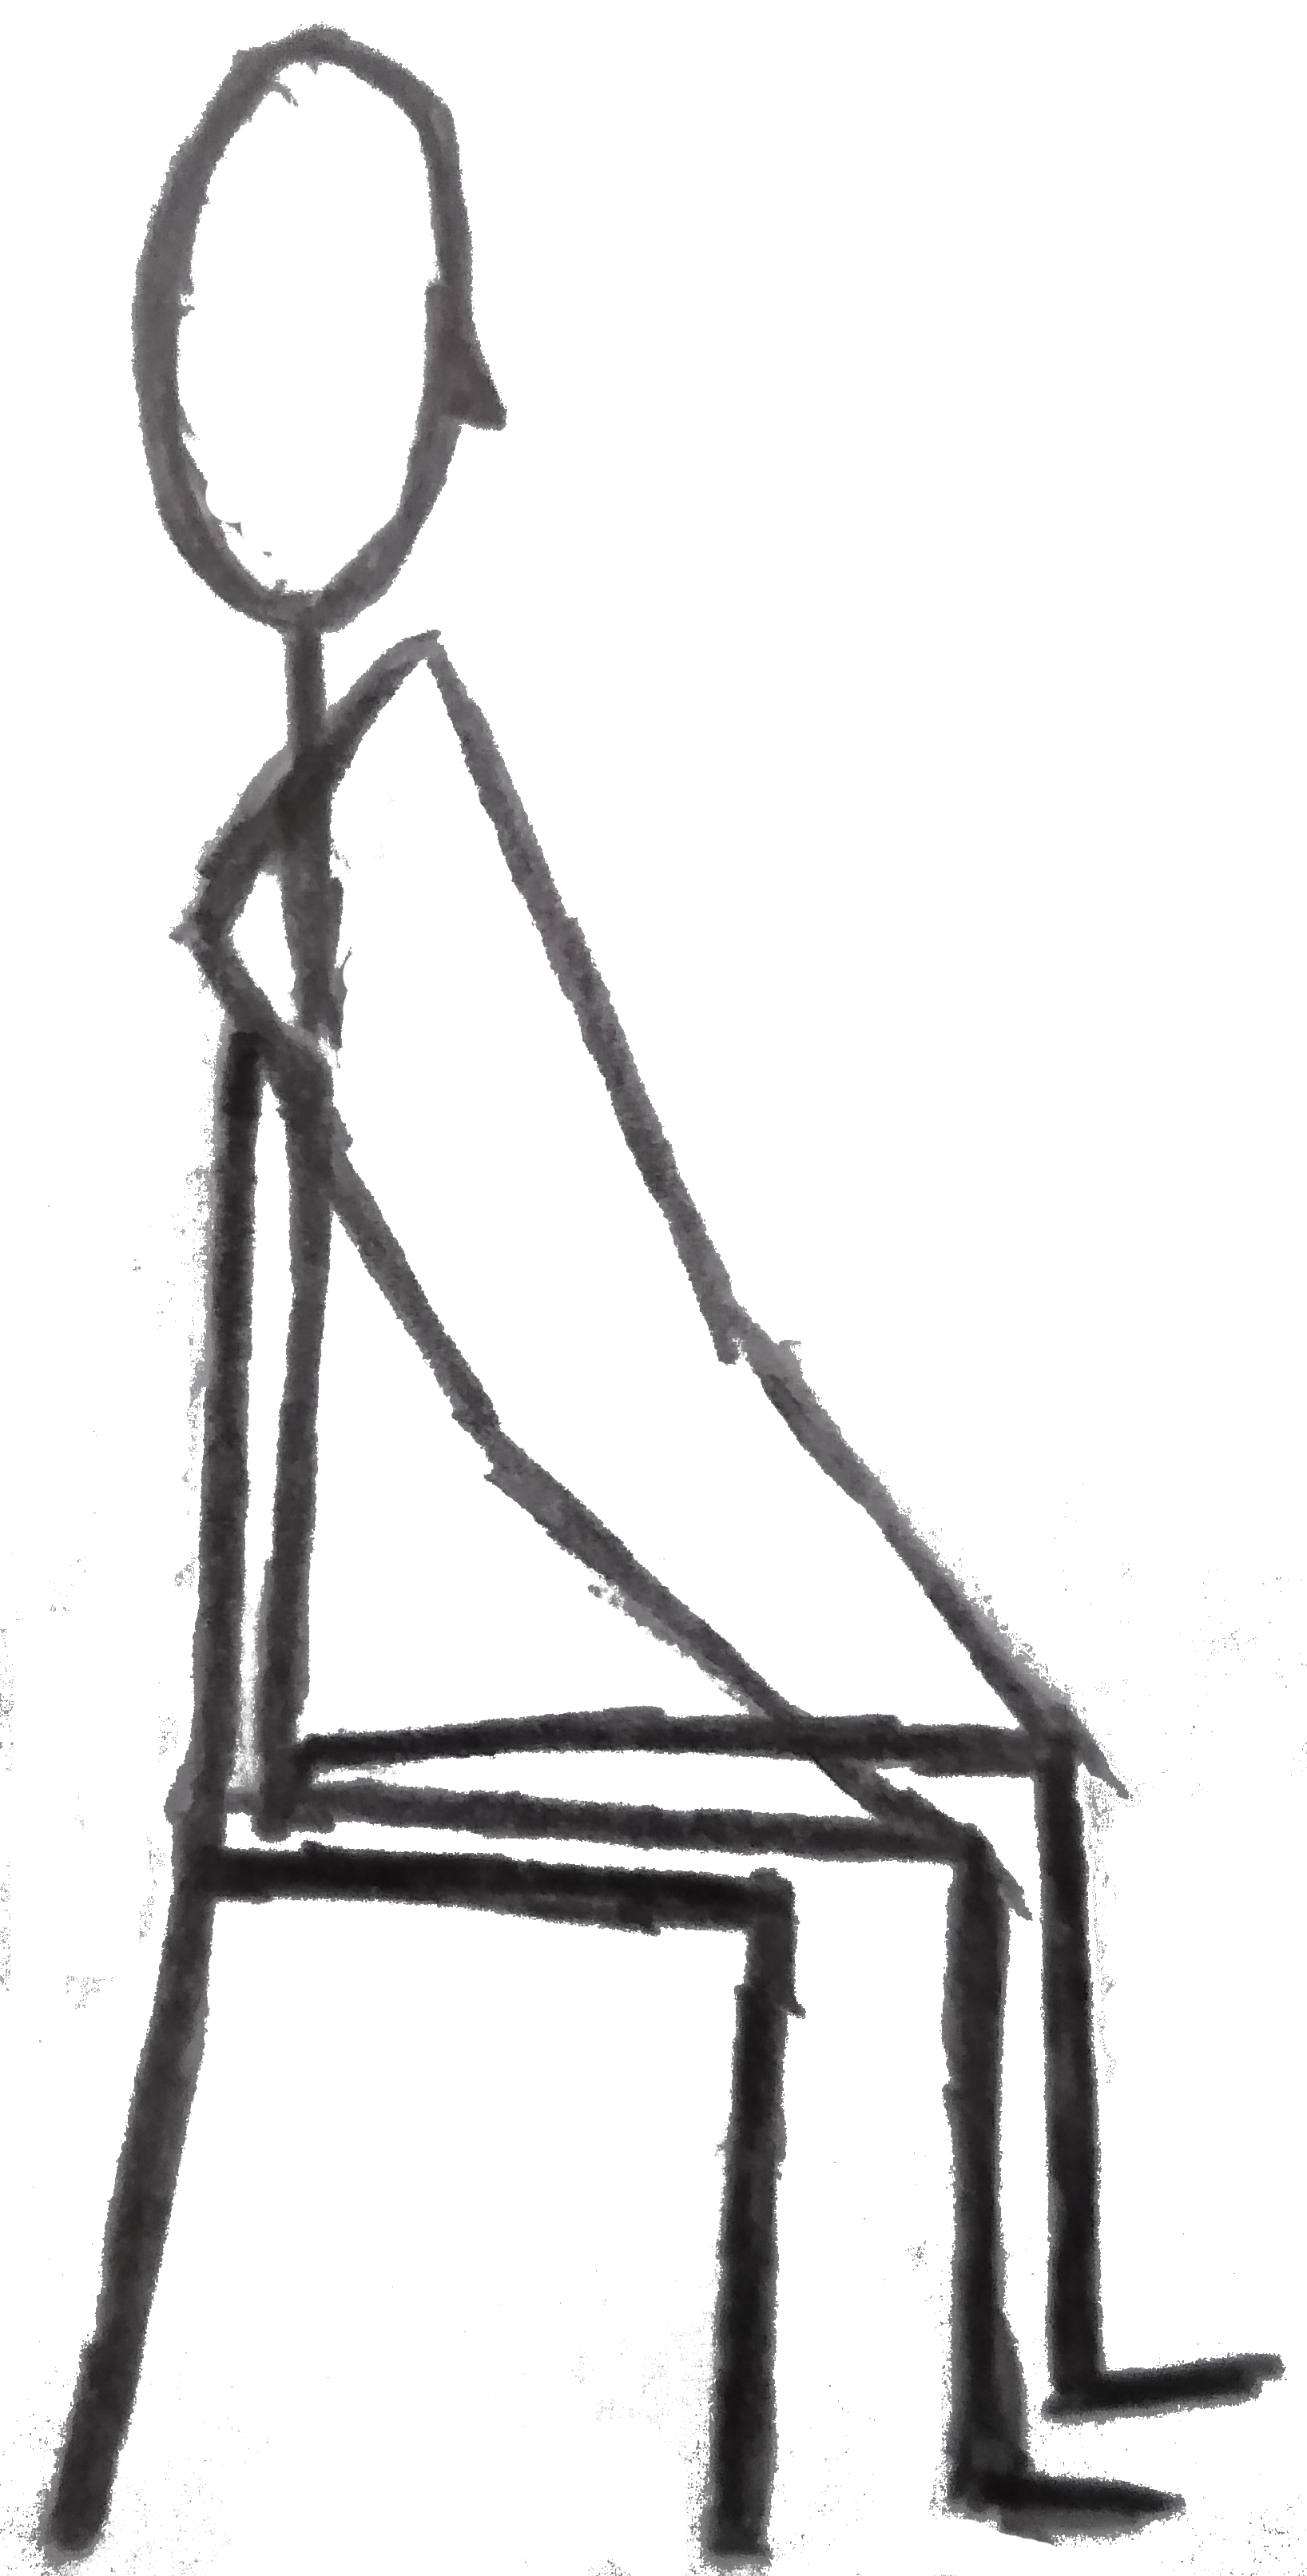
\includegraphics[width=\linewidth]{Sitting_chair_side.png}
%\column{.7\textwidth} % Right column and width

During the body scan, you will \structure{explore the different regions of your body}. \structure{Lie on your back} and focus your attention through your body: bit by bit, from one part to the next, every moment \structure{conscious of your perceptions}.

\structure{Lying on the back}, can be a wonderful form of meditation, as long as you are able to \structure{stay awake}. In order to not doze off, \structure{don't cross your legs} and put your \structure{arms next to your body, palms up}.
%\end{columns}
\end{frame}
%------------------------------------------------------------
%------------------------------------------------------------
\begin{frame}
\frametitle{Do it yourself}
%\begin{columns}[c] % The "c" option specifies centered vertical alignment while the "t" option is used for top vertical alignment

%\column{.3\textwidth} % Left column and width
%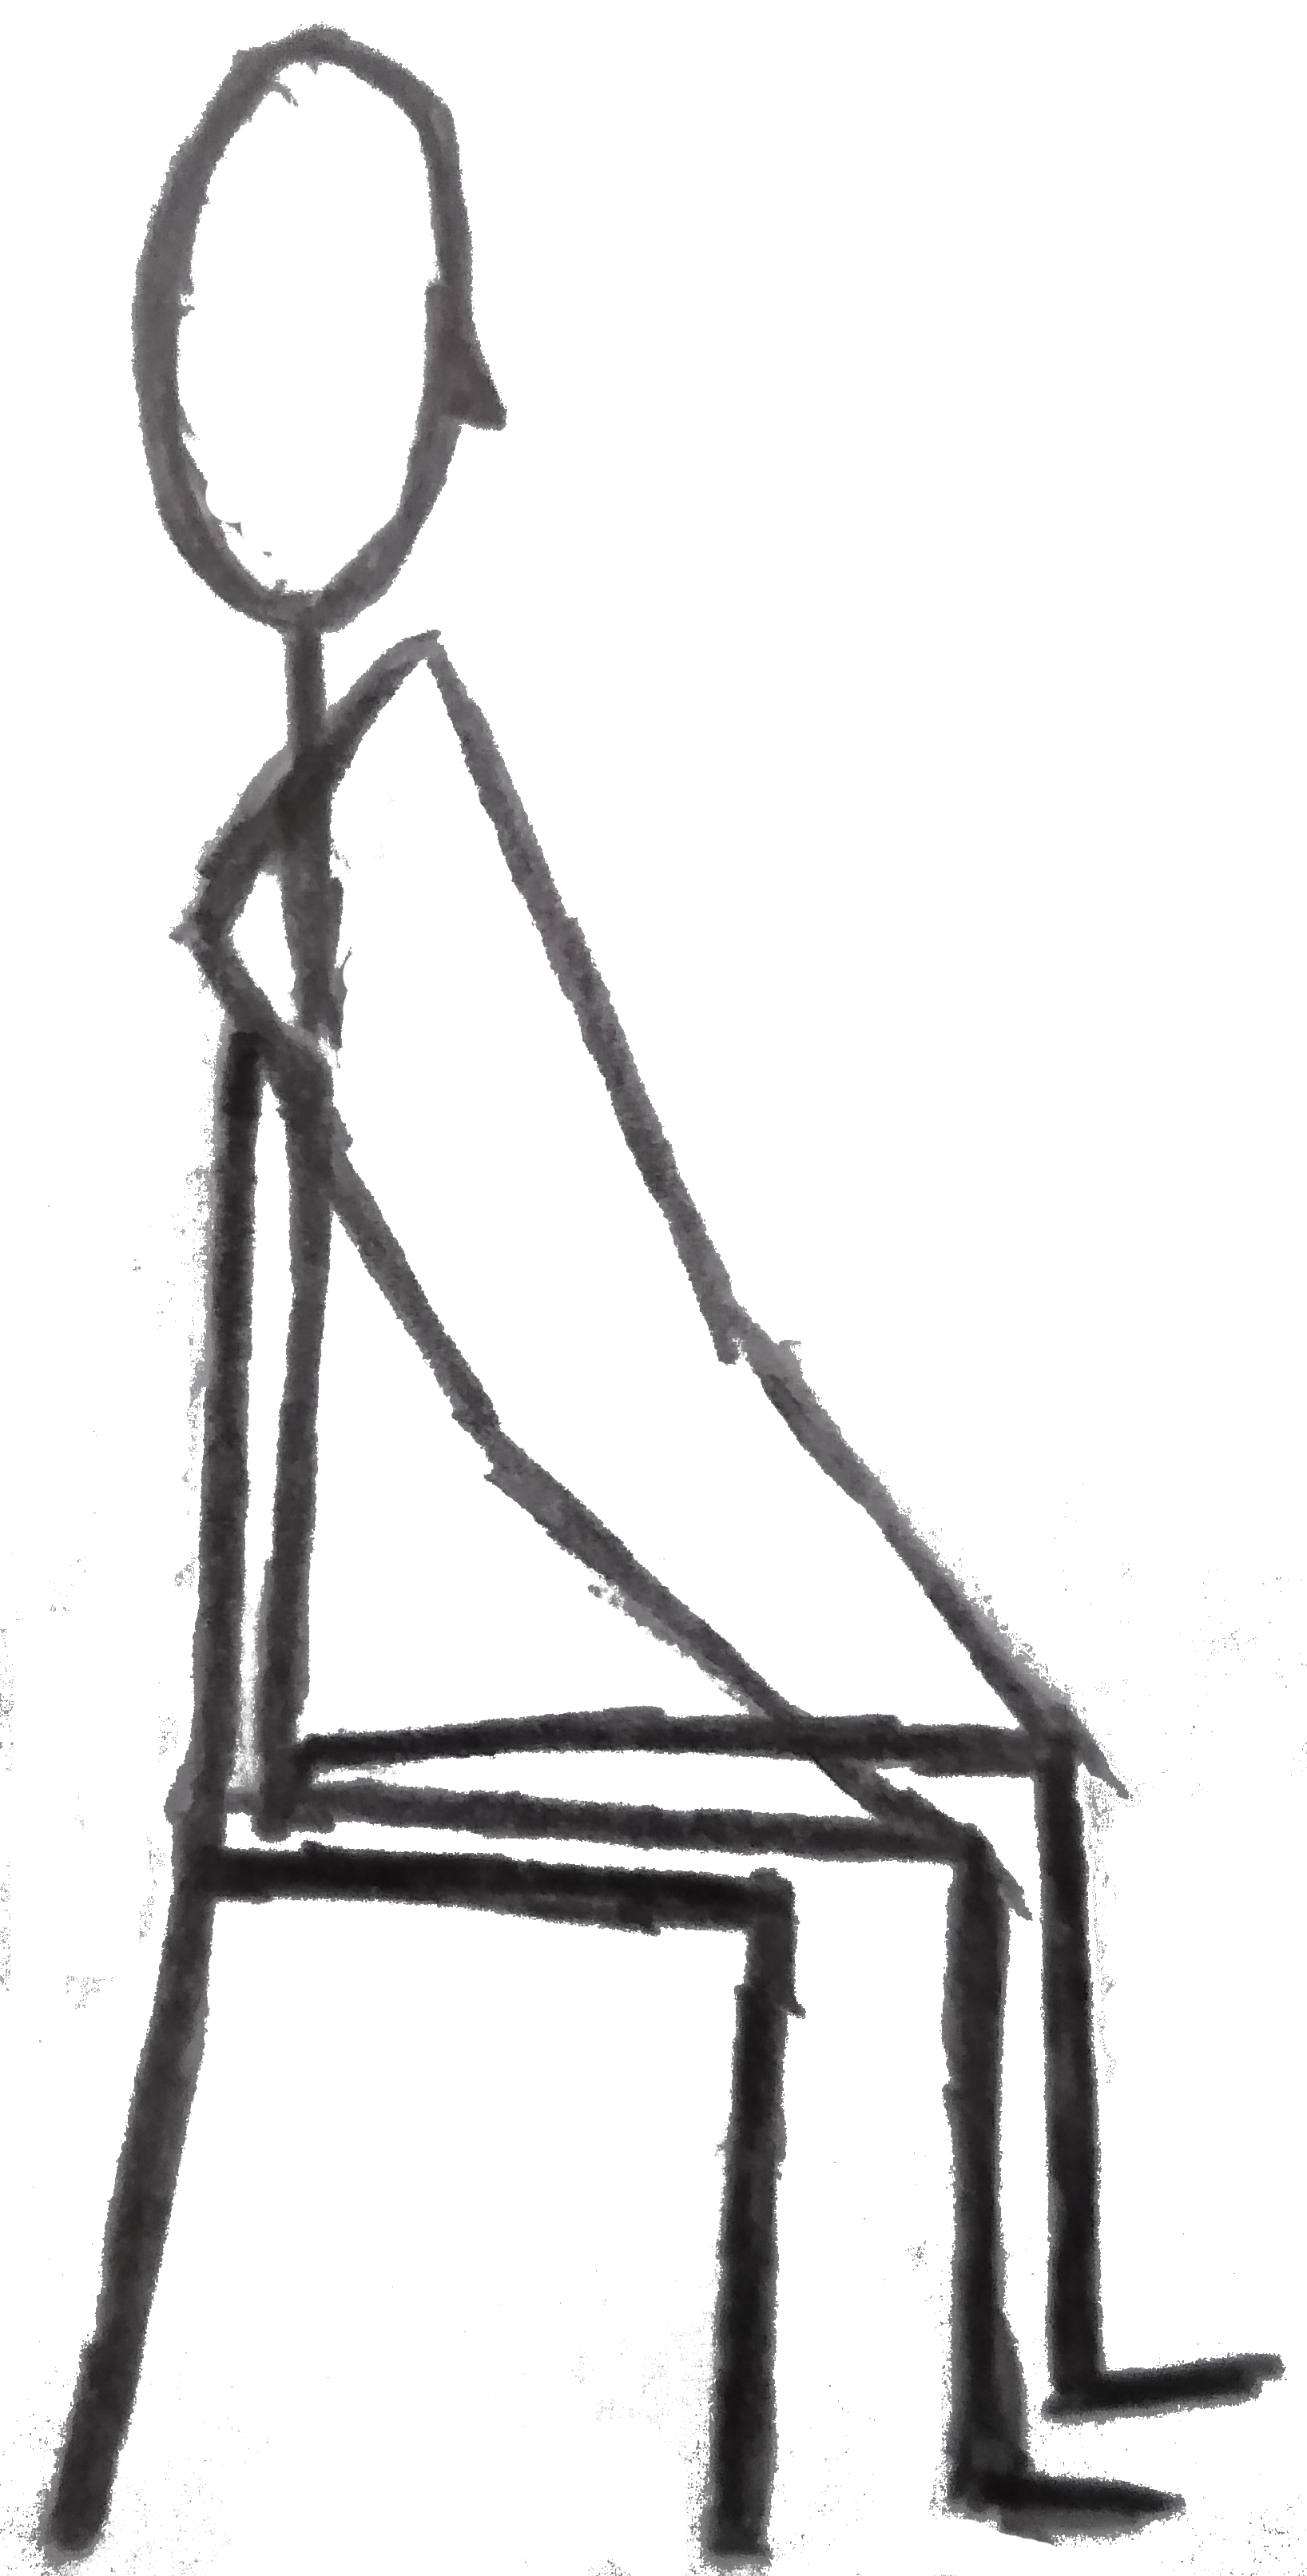
\includegraphics[width=\linewidth]{Sitting_chair_side.png}
%\column{.7\textwidth} % Right column and width

The guided body scan help help you to scan your body to the smallest detail, but you can do that as well yourself with \structure{your own words and thoughts}. 

\structure{From the toes of your left foot, through the foot and the leg to the hip, fro the right toes again to the hip, up through the torso, the loin, the belly, the sacrum, the chest to the shoulders. From the fingers, through the arms to the shoulders, to the face, the back of your head and the crown}.
%\end{columns}
\end{frame}
%------------------------------------------------------------
%------------------------------------------------------------
\begin{frame}
\frametitle{Outcomes}
%\begin{columns}[c] % The "c" option specifies centered vertical alignment while the "t" option is used for top vertical alignment

%\column{.3\textwidth} % Left column and width
%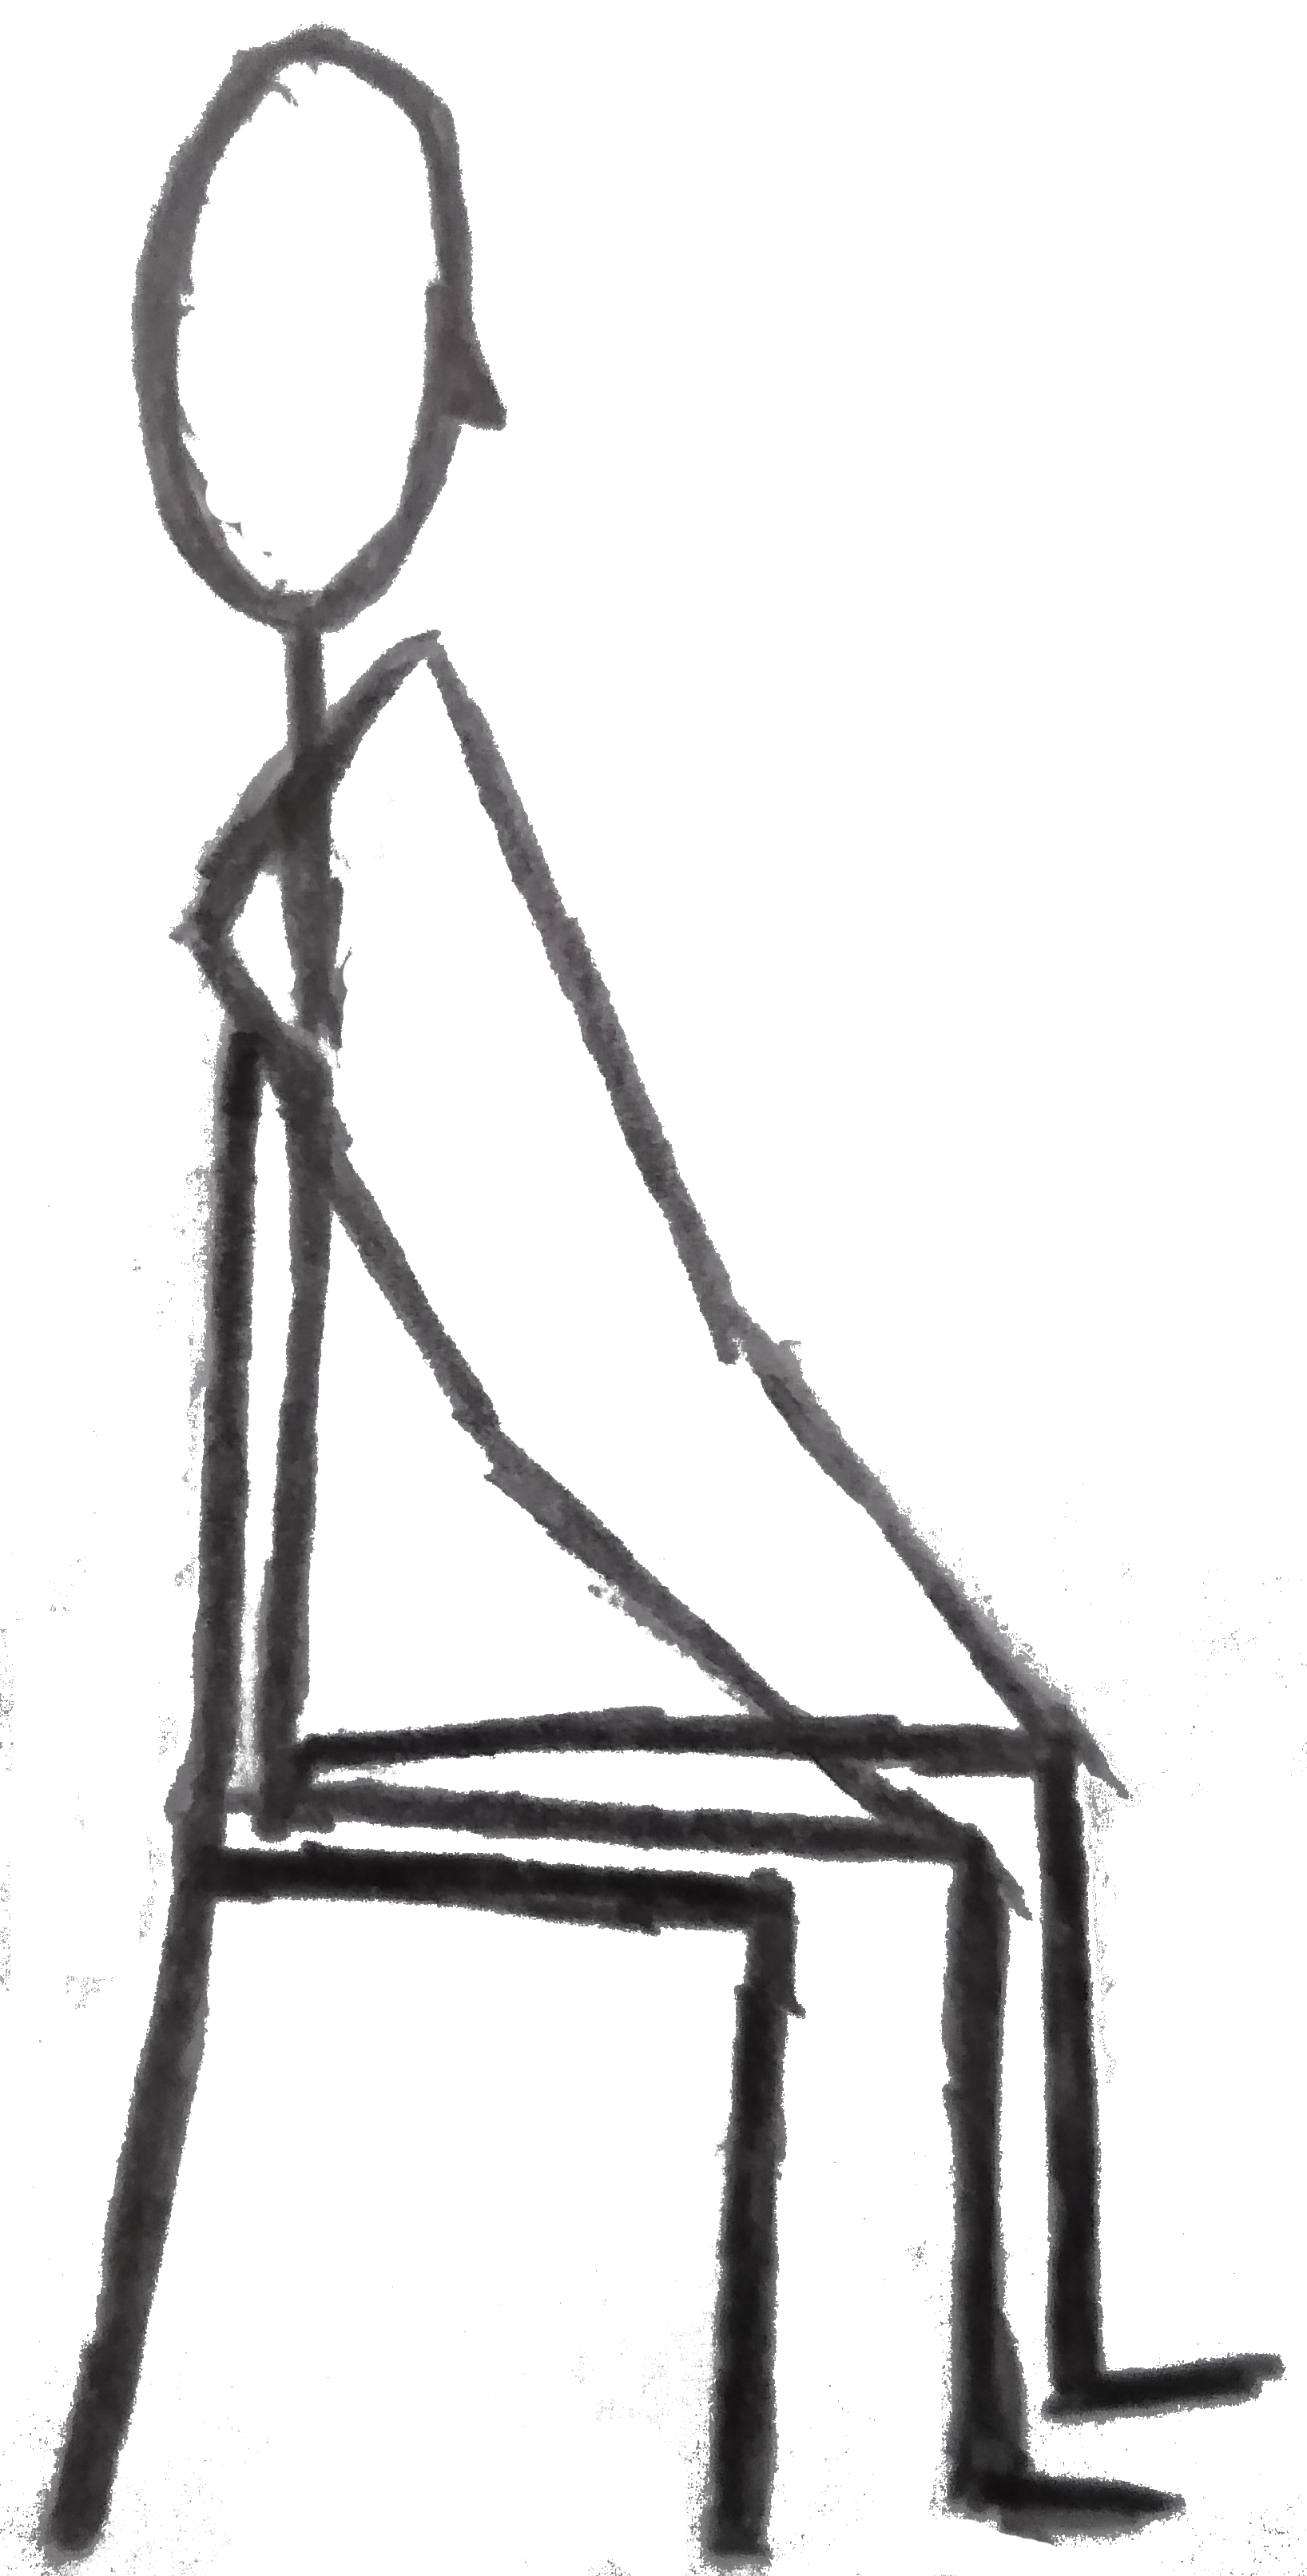
\includegraphics[width=\linewidth]{Sitting_chair_side.png}
%\column{.7\textwidth} % Right column and width

The body scan allows you to \structure{focus your attention} onto a part of your body, to truly feel it and \structure{stay present} in it while \structure{inhaling into and exhaling out of it}. 

It sounds so mundane and yet it may induce \structure{unforeseen outcomes}. By consciously letting go of the habitual bodily sensations and the associated inner pictures and thoughts the muscles are able to \structure{relax} and built--up tensions can be released.
%\end{columns}
\end{frame}
%------------------------------------------------------------
%------------------------------------------------------------
\begin{frame}
\frametitle{Process of cleaning}
%\begin{columns}[c] % The "c" option specifies centered vertical alignment while the "t" option is used for top vertical alignment

%\column{.3\textwidth} % Left column and width
%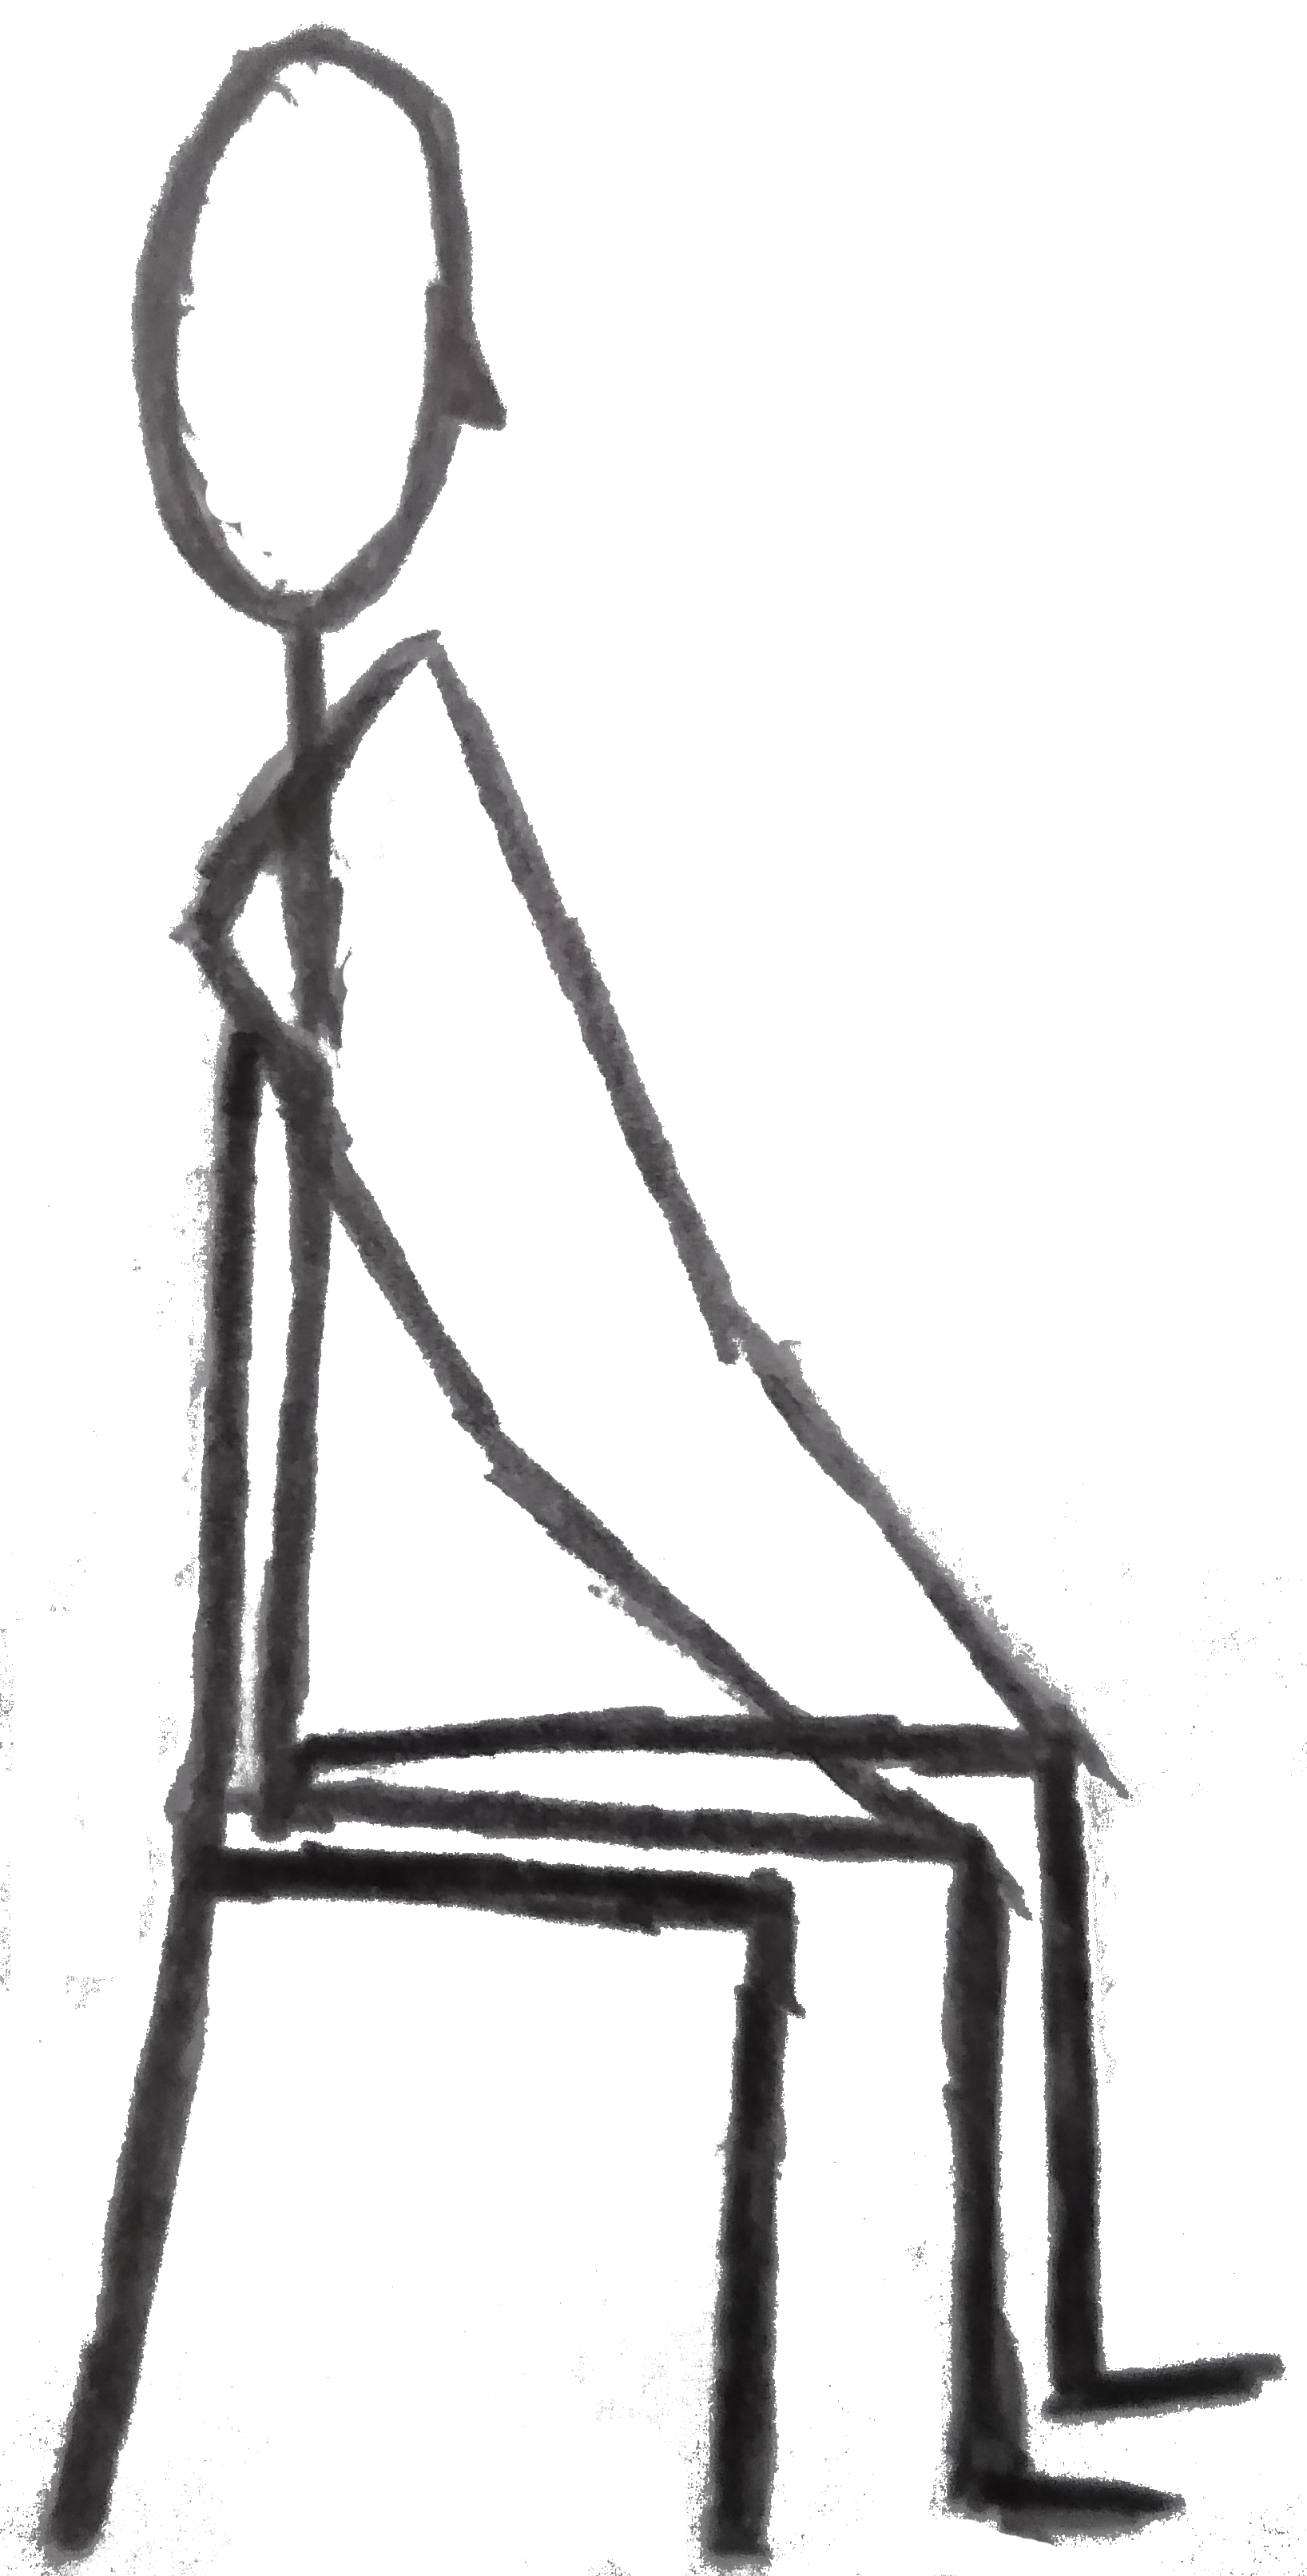
\includegraphics[width=\linewidth]{Sitting_chair_side.png}
%\column{.7\textwidth} % Right column and width
During the body scan, your \structure{attention moves in a narrow focussed zone} along your body and \structure{collects tensions and pains} and transports them up the spine to the crown, where they \structure{get exhaled} to leave a \structure{purified body} behind.

Remember and picture this cleaning and detoxification process while performing the body scan. That may support your efforts and restore in your body a feeling of oneness.

This \structure{cleaning} is important, but you can't force it. Let the cleaning process \structure{take care of itself}. Avoid getting in the situation to anticipate it or to judge it as ``good'' or ``bad'', just continue scanning your body.
%\end{columns}
\end{frame}
%------------------------------------------------------------
%------------------------------------------------------------
\begin{frame}
\frametitle{Reactions to the body scan}
%\begin{columns}[c] % The "c" option specifies centered vertical alignment while the "t" option is used for top vertical alignment

%\column{.3\textwidth} % Left column and width
%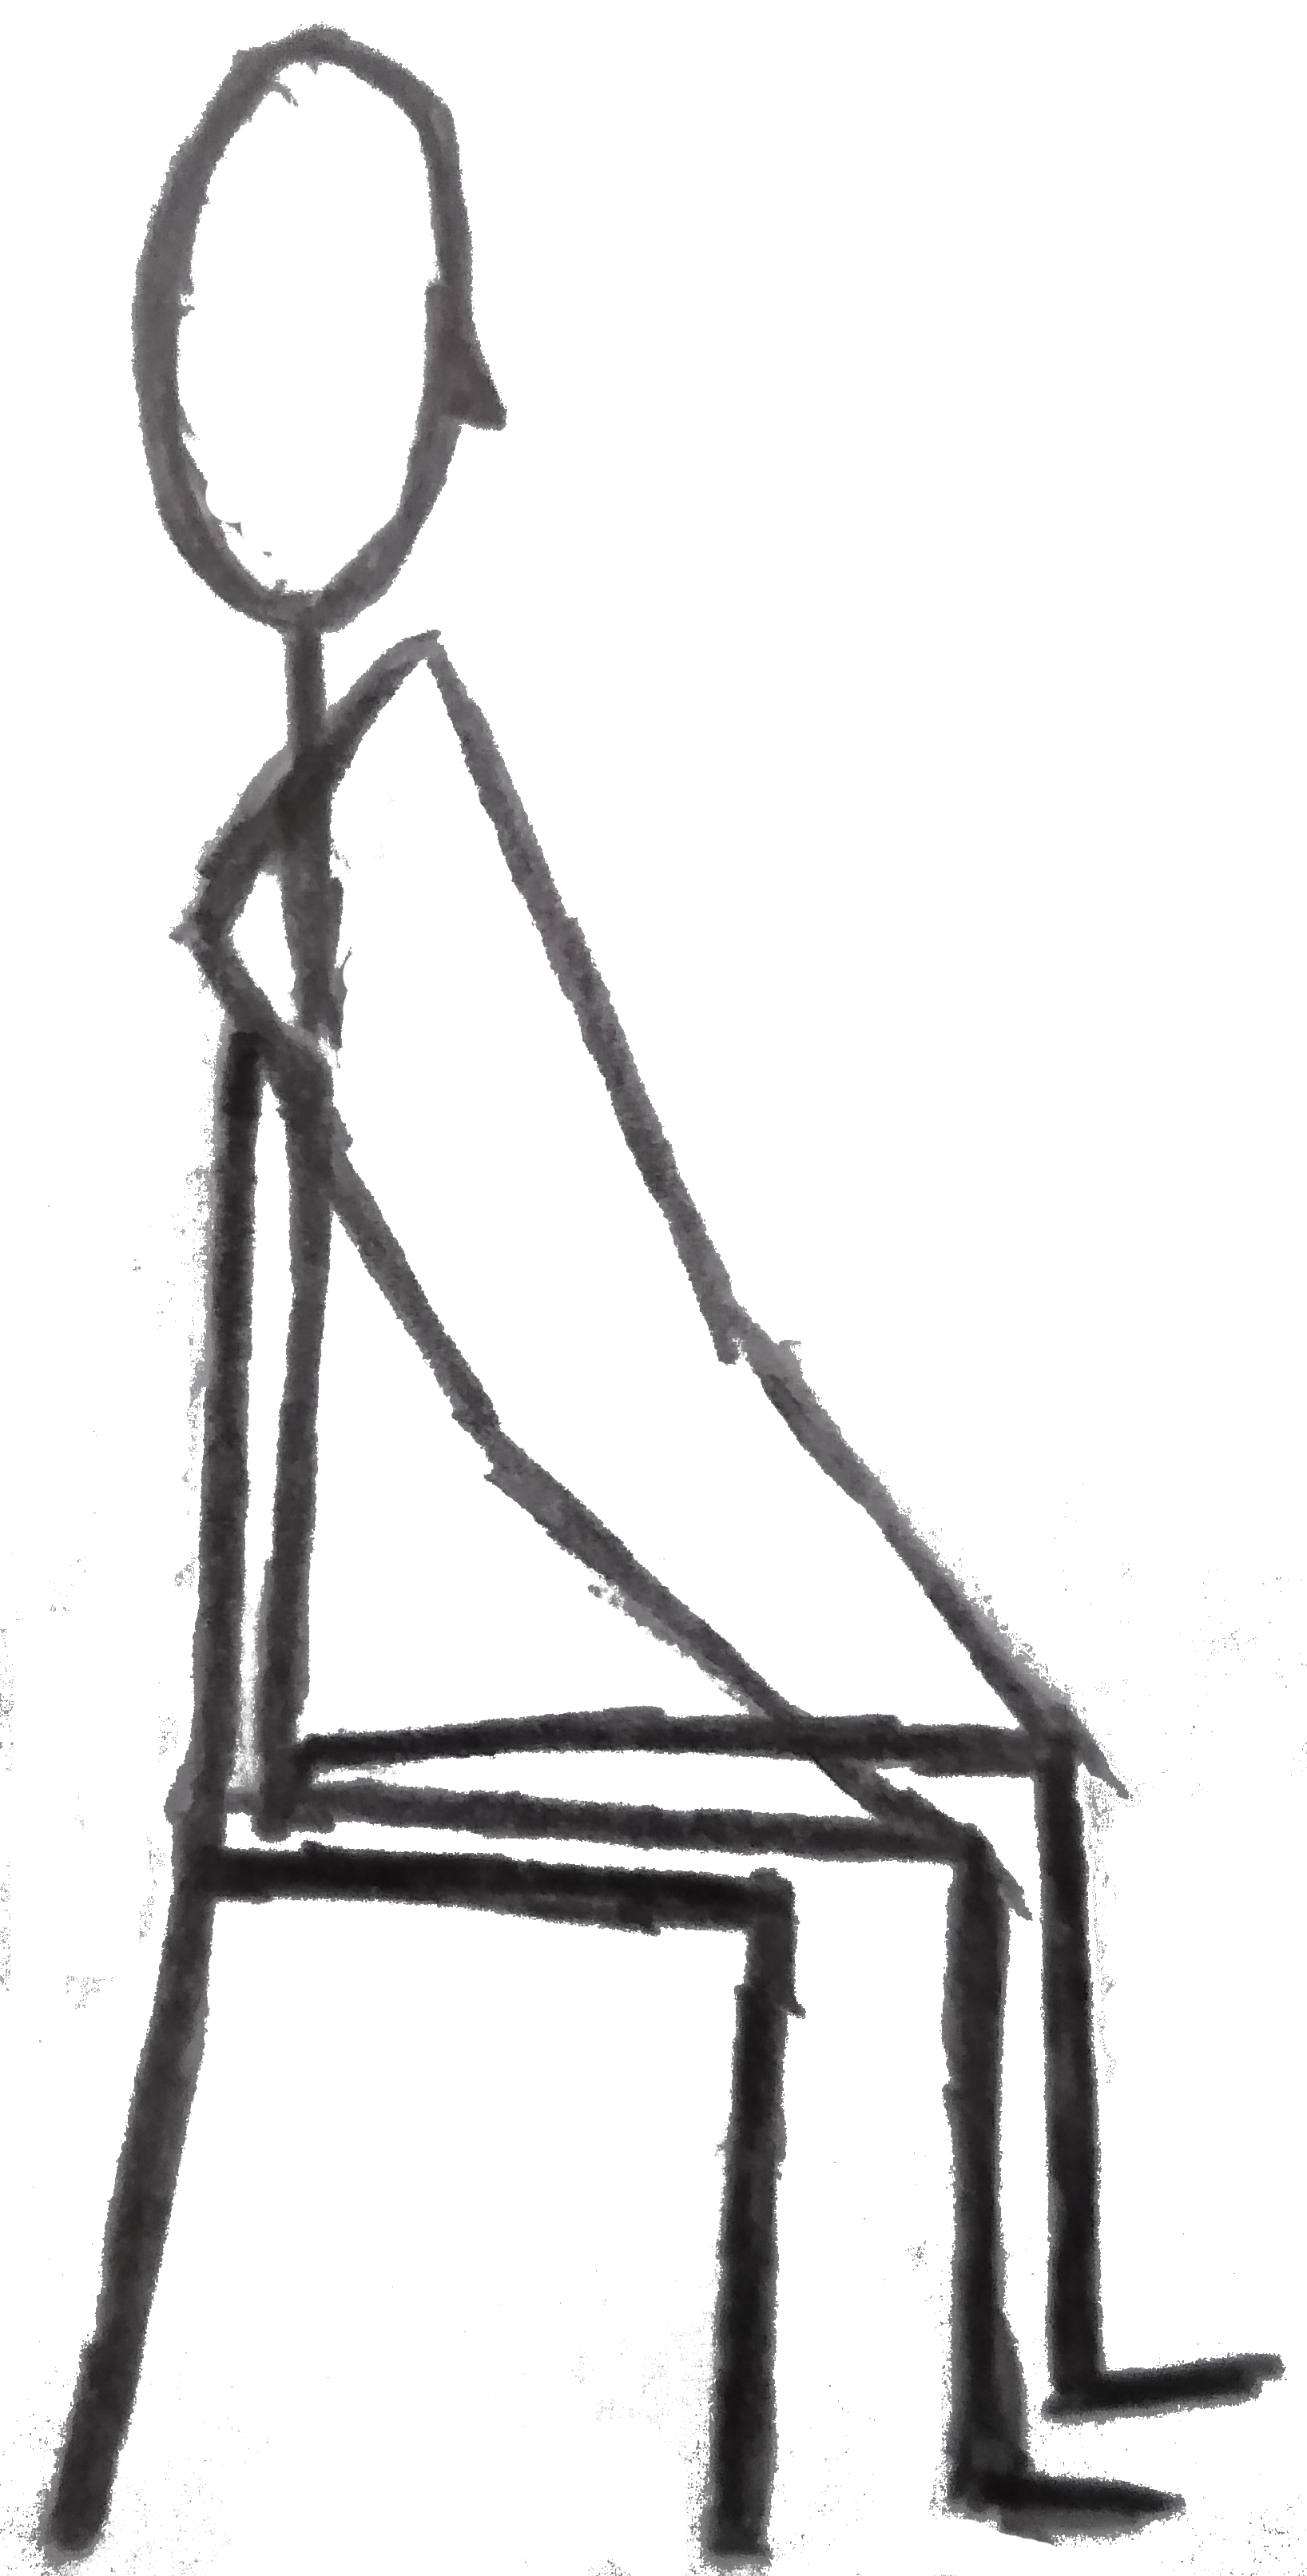
\includegraphics[width=\linewidth]{Sitting_chair_side.png}
%\column{.7\textwidth} % Right column and width
People react in very different ways to the body scan. Some people experience an \structure{inner calm and well--being}, others might experience \structure{increased tensions, pain, anger, boredom, restlessness} or other irritating feelings. 

It doesn't matter if you have positive or negative feelings. What counts, is \structure{your readiness to accompany your feelings with your full attention} --- no matter if they are positive, neutral or negative.
%\end{columns}
\end{frame}
%------------------------------------------------------------
%------------------------------------------------------------
\begin{frame}
\frametitle{Possible side reactions}
%\begin{columns}[c] % The "c" option specifies centered vertical alignment while the "t" option is used for top vertical alignment

%\column{.3\textwidth} % Left column and width
%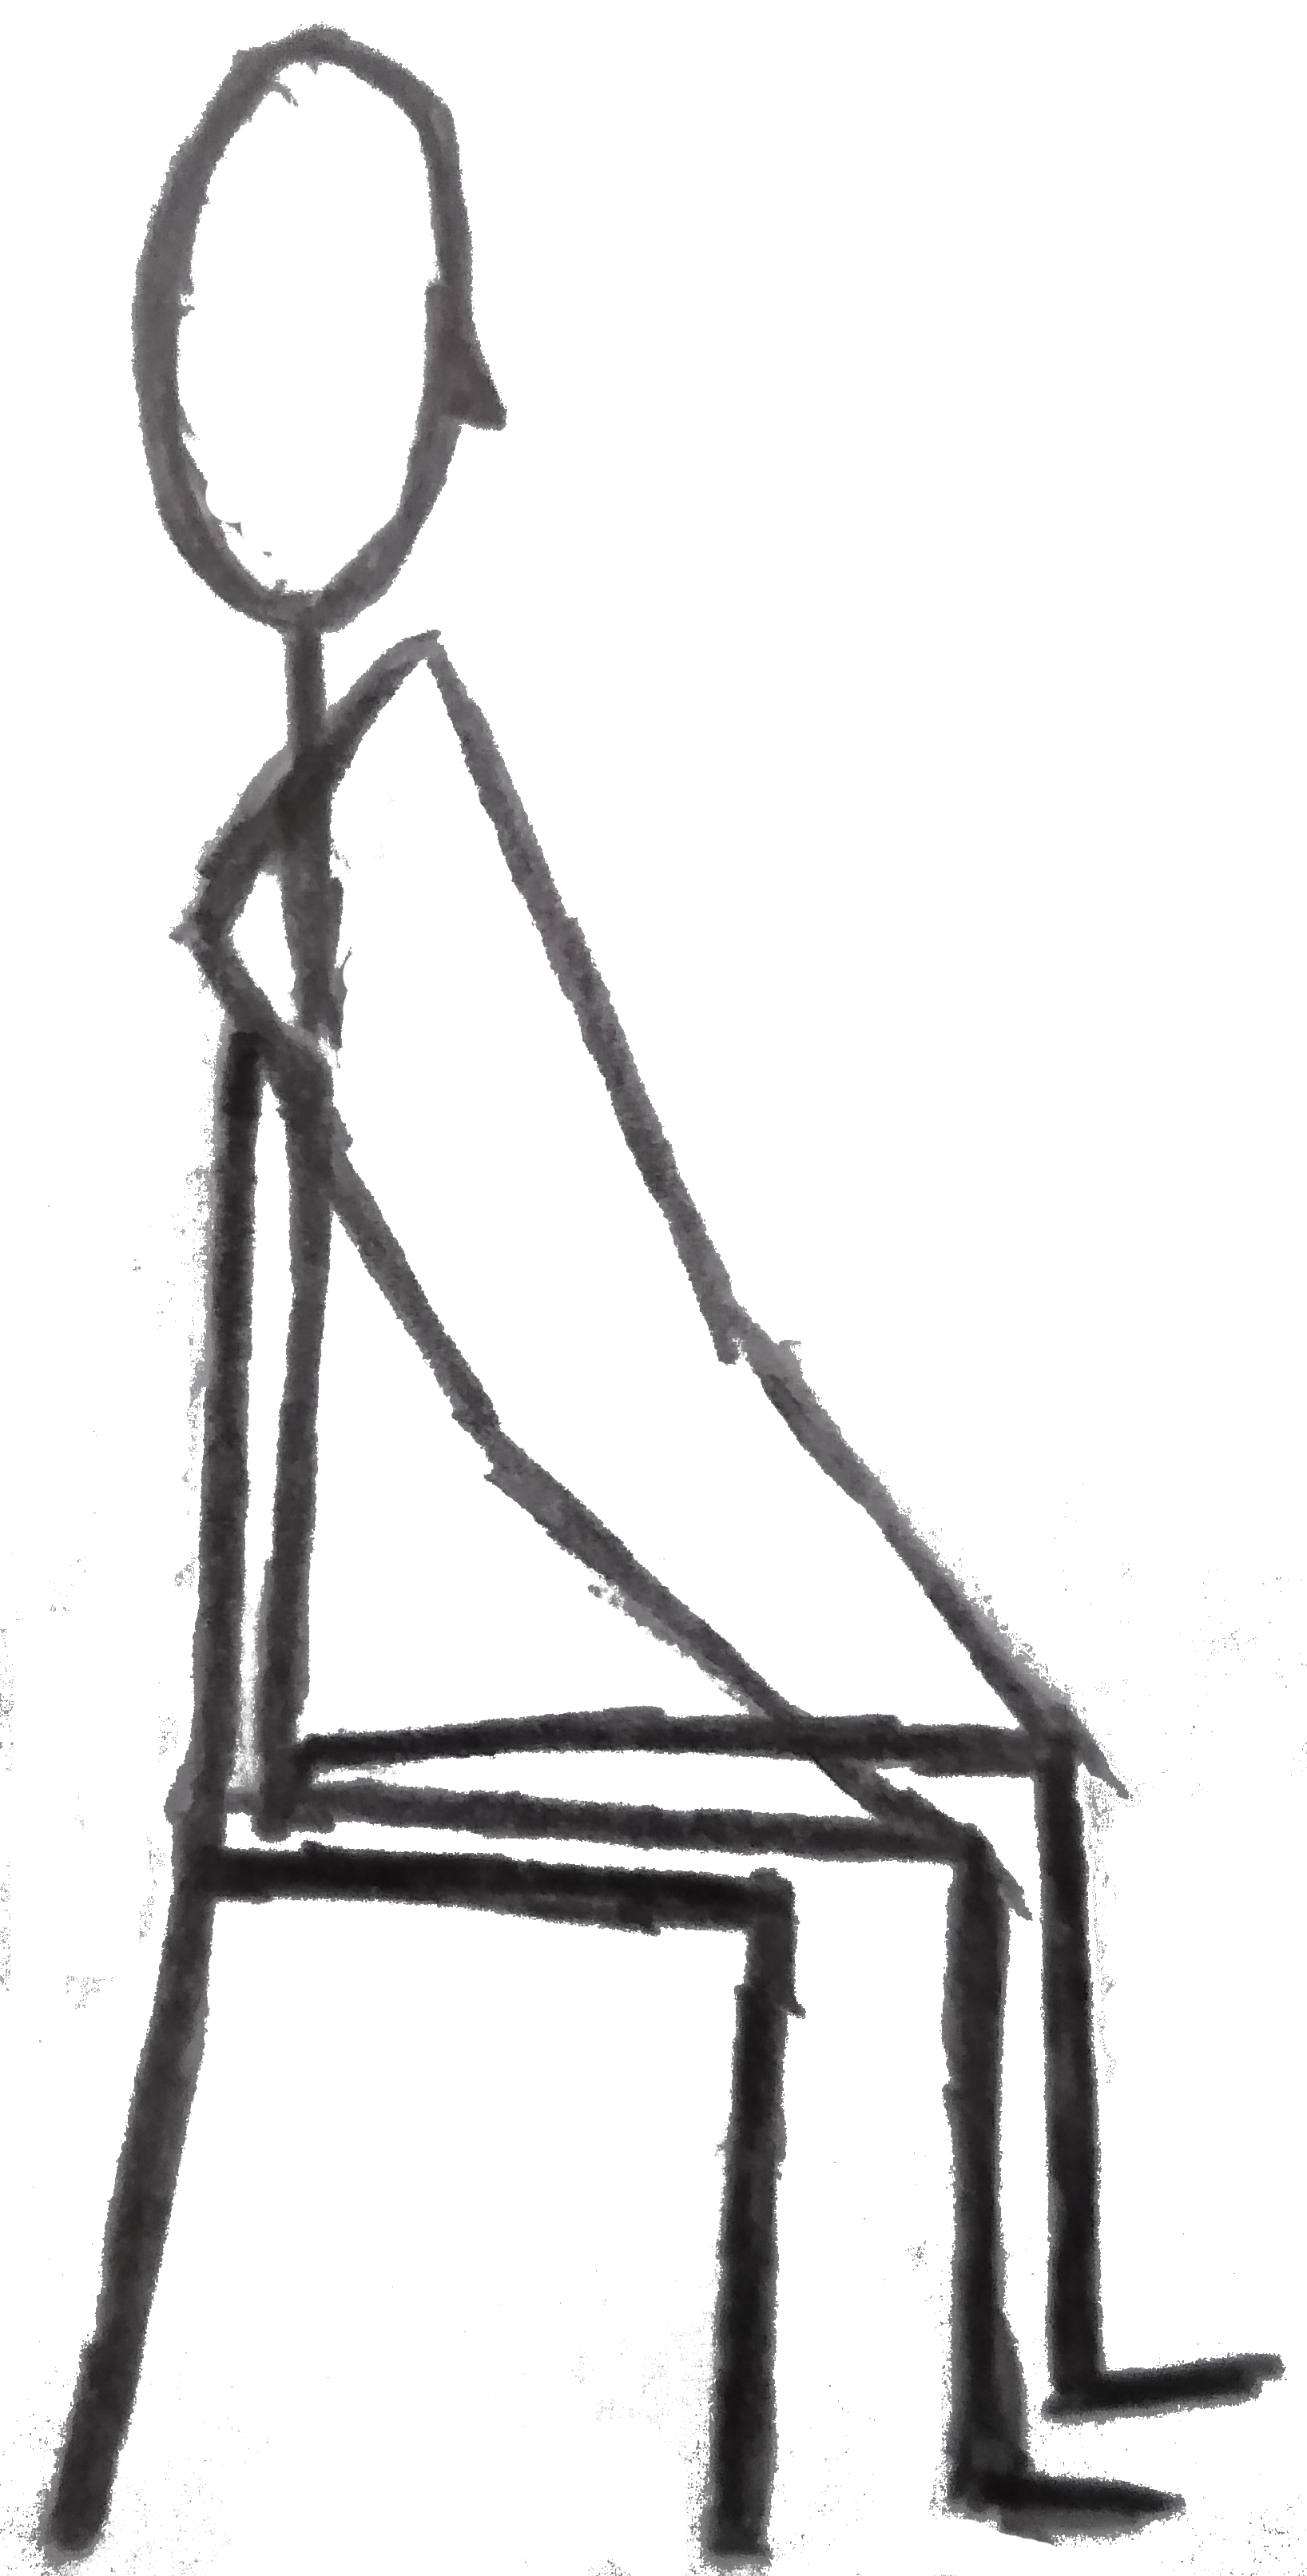
\includegraphics[width=\linewidth]{Sitting_chair_side.png}
%\column{.7\textwidth} % Right column and width
\begin{itemize}
\item[-] Maybe it's hard in the first few hours to \structure{really feel your toes} or other parts of your body,
\item[-] Perhaps you are troubled by \structure{chronic pain or bad feelings}, which distract you and make it \structure{impossible to feel anything else} then the pain or the bad feeling.
\item[-] Maybe you get so \structure{relaxed} while doing the body scan and you \structure{fall asleep}.
\end{itemize}
These and other experiences are \structure{totally normal in the beginning}. Don't get distracted by them. Acknowledge these experiences and \structure{continue practising the body scan}.
%\end{columns}
\end{frame}
%------------------------------------------------------------


